\chapter{Test results}
\label{chap:test_results}

Now that the algorithms have been written about in detail, let me explain how I tested the nodes both in simulator and in real life.

\section{Mapping results}
The aim of the mapping node was to find the moving objects in the environment, based on LIDAR scans, and to separate them from the static parts of the map. The algorithm converted the LIDAR measurements into absolute map points, than created a differential grid - basically a map, with the high values not marking objects like a regular map, but marking movements. The algorithm found the possible dynamic point candidates based on this grid. After the candidates have been selected, the algorithm created groups among the measured points, based on the positions. Relying on these groups being valid, and the assumption that points in the same group must be still or moving in the same direction, speed vectors were calculated for the groups. The groups with speed larger than a minimum value (which may be caused by measurement noise) became the moving objects, and the points inside these groups were marked dynamic. Every other measurement was treated non-moving, and therefore placed in the static map. The static map building is as straightforward as it can be - every static measurement creates a free ray in the map, starting from the position of the LIDAR and ending at the measured point.

The results of the mapping and the separation of static and dynamic points are presented by an example with a valid use-case. The scenario is the following. The car is standing in a closed room, the distance from the walls are smaller than the LIDAR's range. There is one other object in the room, in the simulation, this is a ball, its size similar to the car's. The ball is standing in one place at first, but after a while, it start moving in a straight path with constant speed. Finally, the car starts moving as well - first in a straight path, then turning.

\ref{mapping_demo_start} presents the initial situation of the demonstration. The left image shows the simulation - the car is standing in the middle of the room, the object in the top left corner is not moving yet. On the right image, the created static map is visible. The number of unknown (grey) grid points is large at this state of the simulation, it will dramatically decrease once the car starts moving. This effect is caused by the LIDAR's finite angular resolution and ray characteristics. The black grid points represent statically occupied positions. All the walls are marked static, and the ball as well.

\begin{figure}[!ht]
    \centering
    \subfloat[Gazebo simulation]
    {
        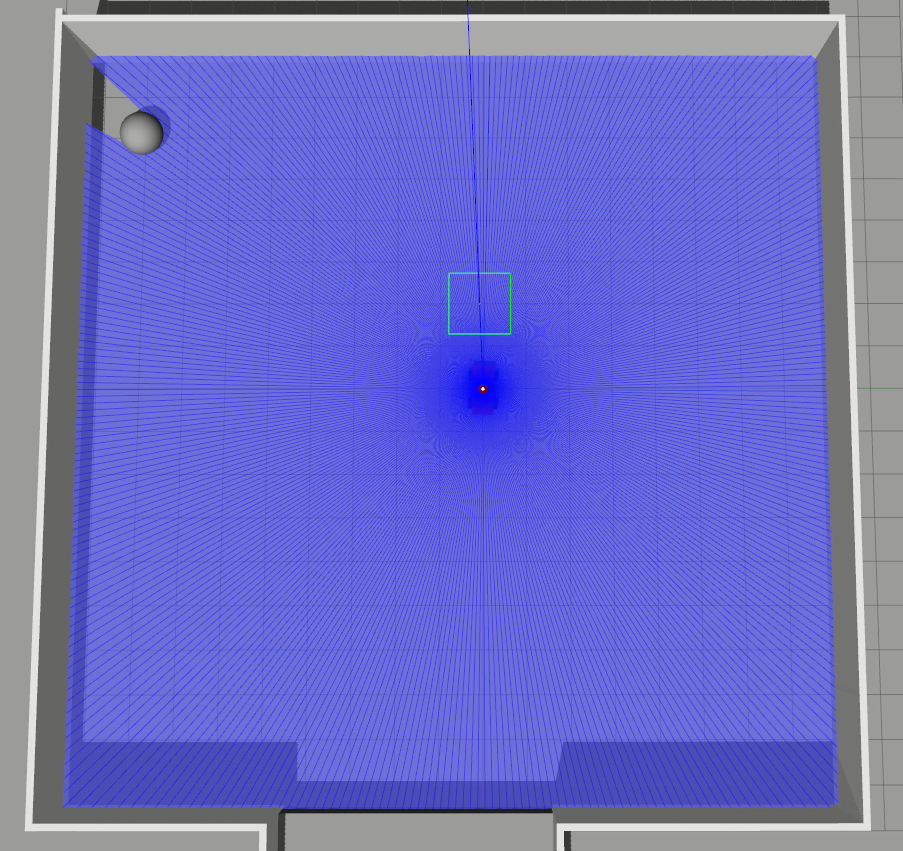
\includegraphics[height=70mm]{figures/raw/mapping_demo/gazebo_start.png}
        \label{mapping_demo_gazebo_start}
    }
    \subfloat[rviz visualization]
    {
    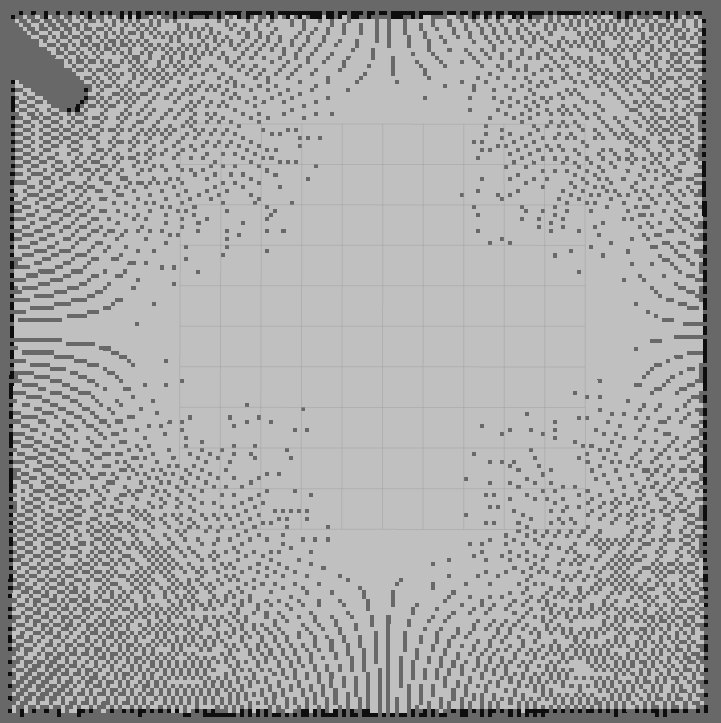
\includegraphics[height=70mm]{figures/raw/mapping_demo/rviz_start.png}
        \label{mapping_demo_rviz_start}
    }
    \caption{Initial state - ball is still}
    \label{mapping_demo_start}
\end{figure}

Once the ball starts moving (\ref{mapping_demo_ball_moving}), it stops being marked as static, but is handled as a moving object. The static block at the top left corner has been removed, and the ball is displayed using the dynamic visualization toolset - a sphere and an arrow, representing the ball's area and speed vector.

\begin{figure}[!ht]
    \centering
    \subfloat[Gazebo simulation]
    {
        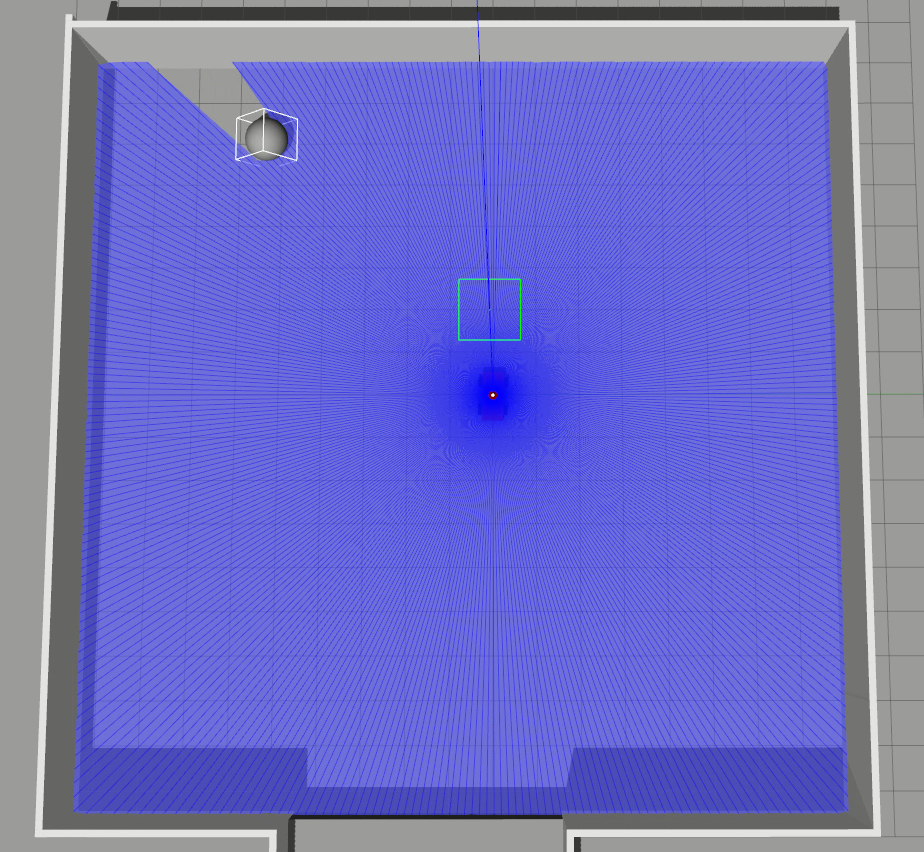
\includegraphics[height=70mm]{figures/raw/mapping_demo/gazebo_ball_moving.png}
        \label{mapping_demo_gazebo_ball_moving}
    }
    \subfloat[rviz visualization]
    {
    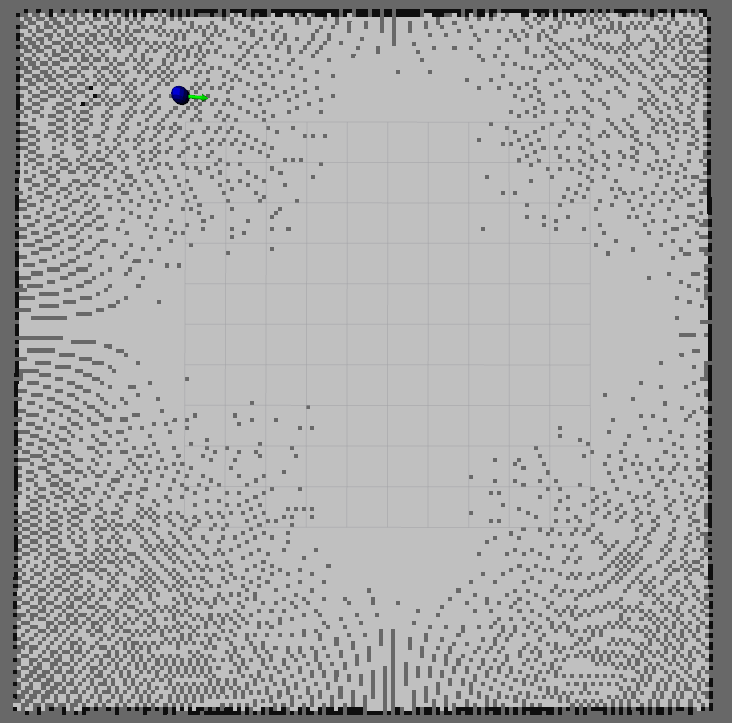
\includegraphics[height=70mm]{figures/raw/mapping_demo/rviz_ball_moving.png}
        \label{mapping_demo_rviz_ball_moving}
    }
    \caption{The ball is moving}
    \label{mapping_demo_ball_moving}
\end{figure}

When the car starts moving, the map immediately starts to clear out. If we compare \ref{mapping_demo_ball_moving} and \ref{mapping_demo_car_moving}, it is clear that the latter contains less unknown grid points.

\begin{figure}[!ht]
    \centering
    \subfloat[Gazebo simulation]
    {
        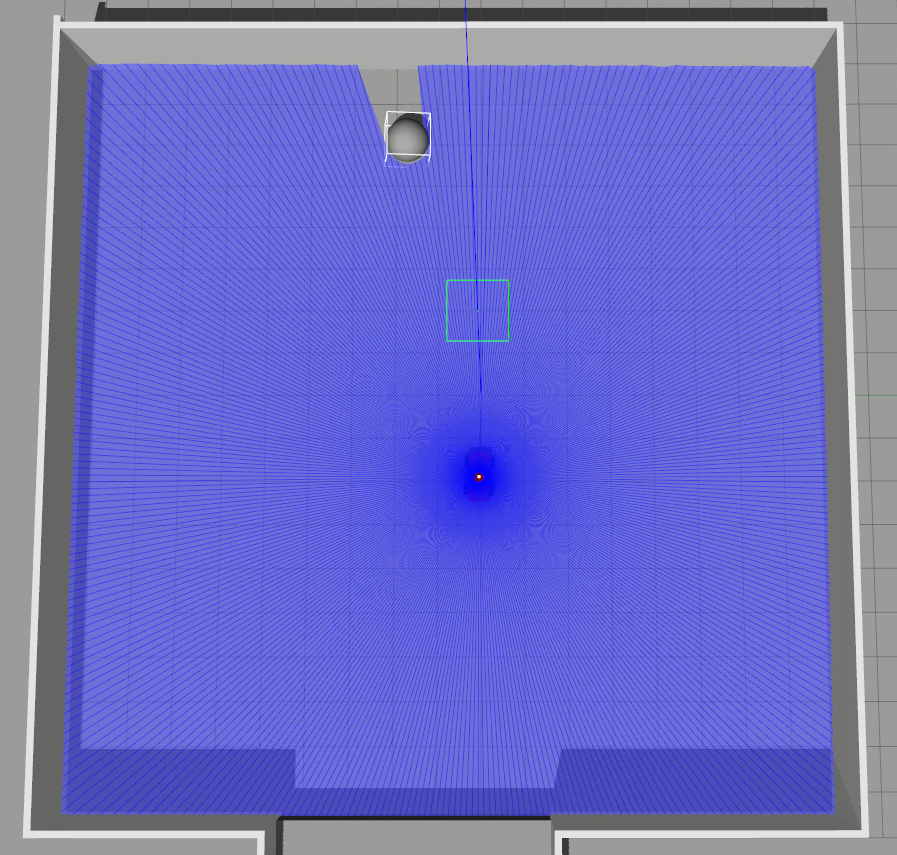
\includegraphics[height=70mm]{figures/raw/mapping_demo/gazebo_car_moving.png}
        \label{mapping_demo_gazebo_car_moving}
    }
    \subfloat[rviz visualization]
    {
    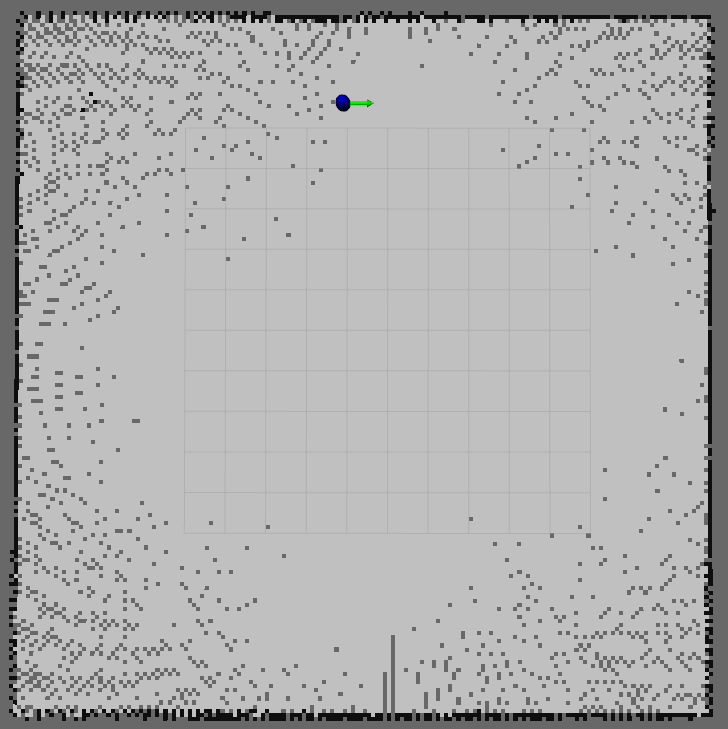
\includegraphics[height=70mm]{figures/raw/mapping_demo/rviz_car_moving.png}
        \label{mapping_demo_rviz_car_moving}
    }
    \caption{The car is moving}
    \label{mapping_demo_car_moving}
\end{figure}

Due to the map implementation being very simple, and updating each map point without handling its history, the mapping node can only be used with certain limitations regarding obstacle speed and the car's angular velocity. But the main task for the mapping algorithm was not to create a static map with the best possible quality, but to separate the static points from the dynamic objects.

\section{Motion planning results}
The task of the motion planning node was to calculate and publish actuations based on the static and dynamic maps provided by the mapping node, that lead the car towards the destination, following the required trajectory, without any collisions. The algorithm first filters the static and dynamic input maps to decrease the number of environment points. Then it calculates trajectories for the dynamic obstacles. Independently from the maps, it sets the target actuation according to the target trajectory or an external control command, and also updates the dynamic window, based on the current actuation. When all these steps are finished, it calculates the collision times for all the actuations in the dynamic window and all objects in the car's environment, and builds the velocity obstacle map. Using this map and the target actuation, fitness factors are calculated for all available actuations. Summarizing and evaluating these factors, the best possible actuation is determined. This actuation is then published to the actuator nodes.

As the motion planning examples also demonstrate the map building implicitly, I recorded several measurements of different kinds of scenarios, and I selected a set of them that represent the algorithms advantages and deficiencies. Most of the scenarios I tested in simulation.

\subsection{Simulator testing}
As a 0th step, I tested if the algorithm follows a straight, then a curved trajectory with no obstacles in the way. These tests were needed to check if actuation handling and the target position update mechanism work as expected. After these features were tested successfully, the testing procedure could move forward to moving objects in the trajectories.

The first example is still a quite simple one. The car is given a straight trajectory, but there is a static obstacle in its way. The expected behaviour is to bypass the object while staying as close to the trajectory as possible, and when the car has moved past the obstacle, it should keep to the trajectory again.

\begin{minipage}{\textwidth}
	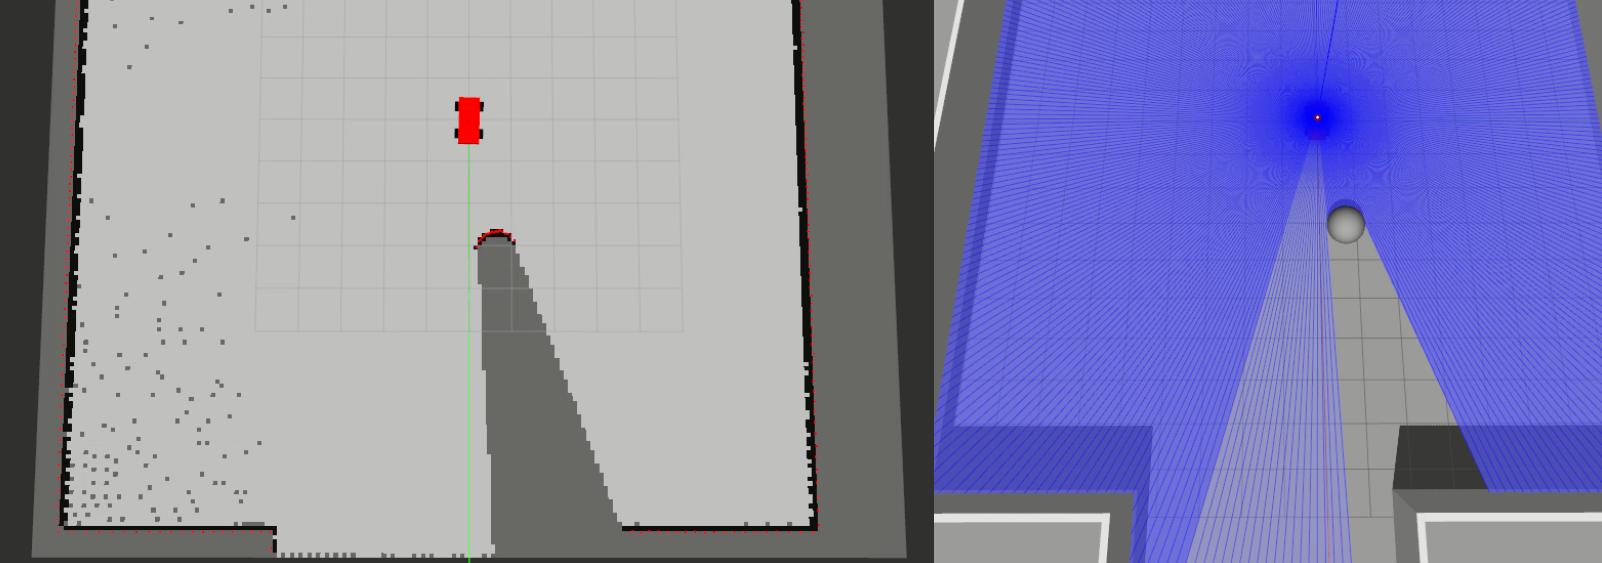
\includegraphics[width=\textwidth]{figures/raw/local_planner_test_straight_traj_static_obj_1.png}

	\vspace{0.5cm}
	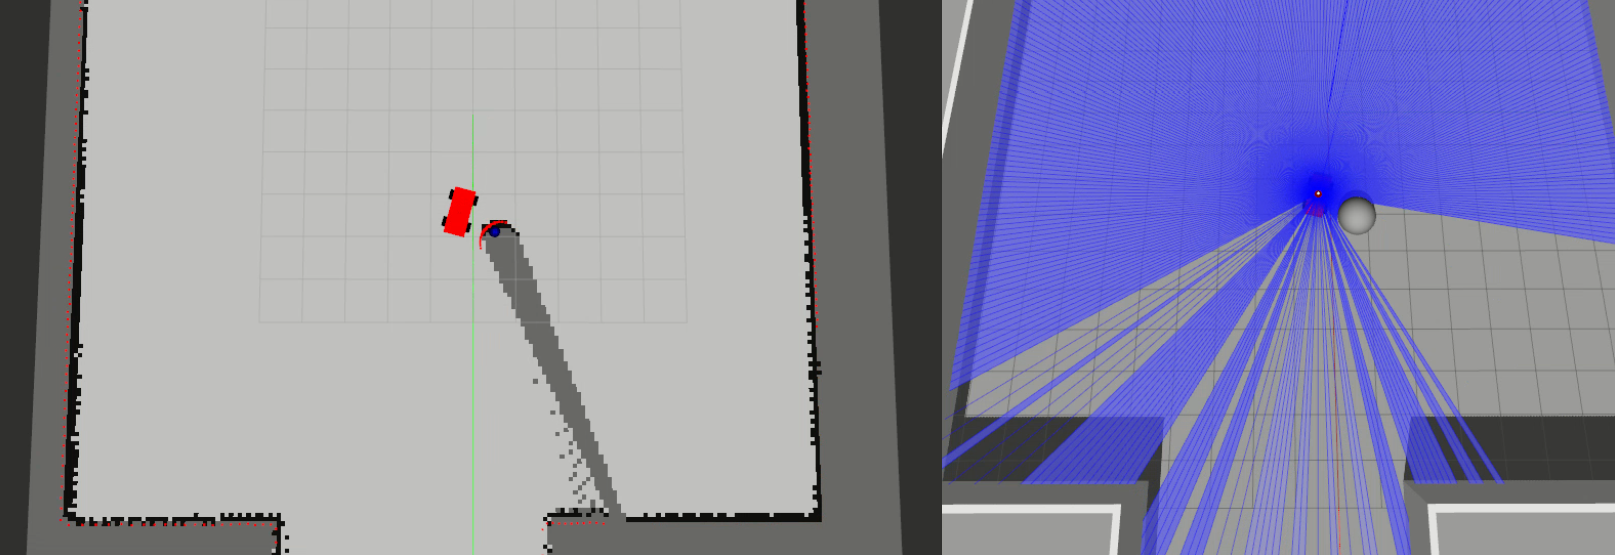
\includegraphics[width=\textwidth]{figures/raw/local_planner_test_straight_traj_static_obj_2.png}

	\vspace{0.5cm}
	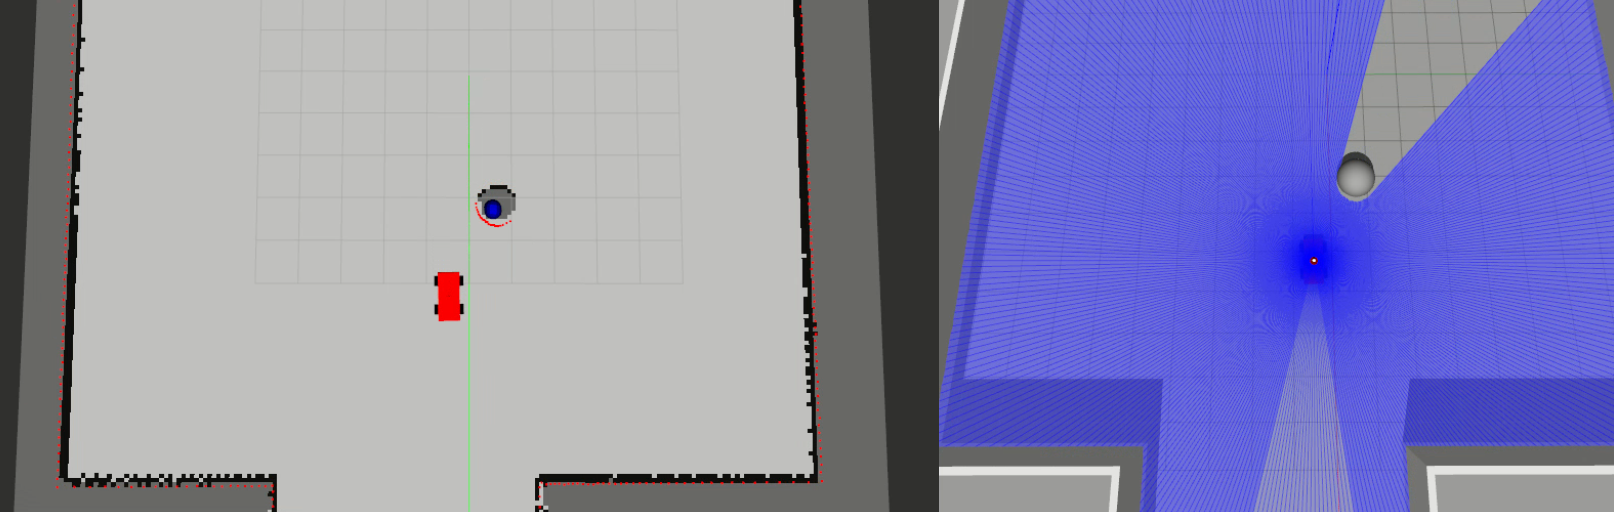
\includegraphics[width=\textwidth]{figures/raw/local_planner_test_straight_traj_static_obj_3.png}

	\vspace{0.5cm}
	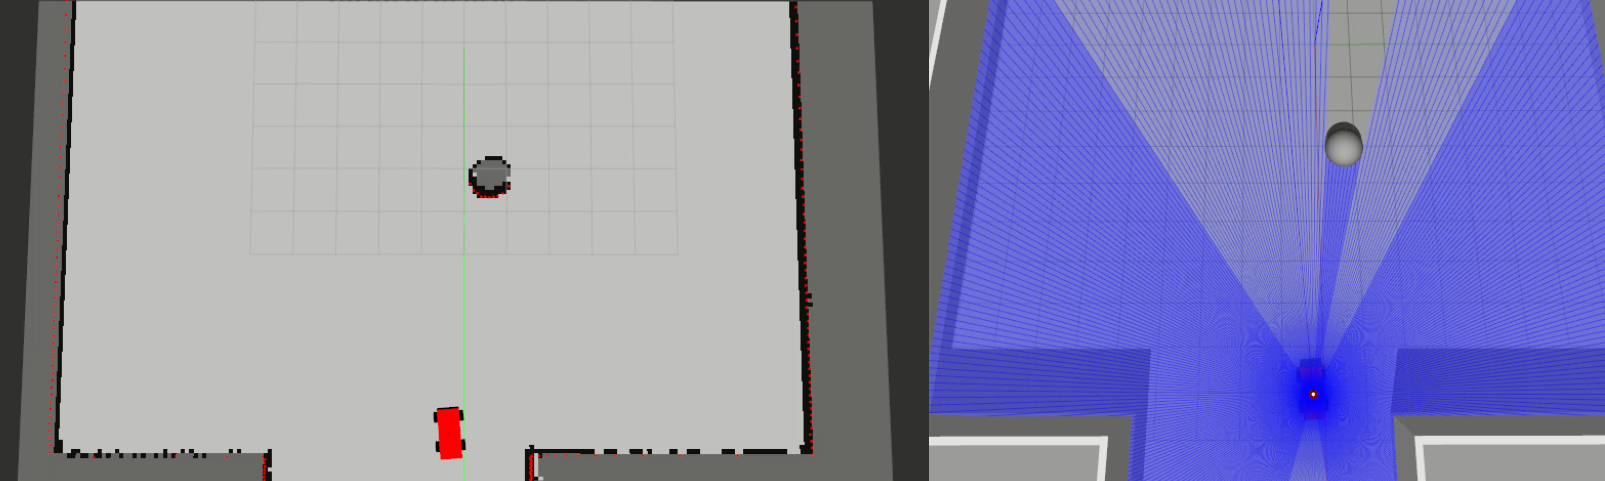
\includegraphics[width=\textwidth]{figures/raw/local_planner_test_straight_traj_static_obj_4.png}

	\captionof{figure}{Straight trajectory, static obstacle}
	\label{local_planner_test_straight_traj_static_obj}
\end{minipage}

The simulation images always display the Gazebo simulation on the right and the rviz visualization on the left. Let me briefly summarize how the objects are displayed in rviz. The car has red colour, the target trajectory is marked by the green line. The LIDAR scan consists of the red dots and the map points are either white (free), grey (unknown) or black (occupied). Therefore, static objects appear as black masses in the map. Each dynamic object is marked with a blue circle representing its position and size, and a green arrow for its speed vector. The car's target trajectory is always pointing downwards, therefore in every test cases the car is trying to navigate to the bottom of the page.

As the image series \ref{local_planner_test_straight_traj_static_obj} show, the car successfully avoids the object and then keeps to the trajectory again.

The second example is similar to the first one, but has one major difference: the object to avoid is not static but is moving opposite the car, with a speed nearly equal to the car's.

\begin{minipage}{\textwidth}
	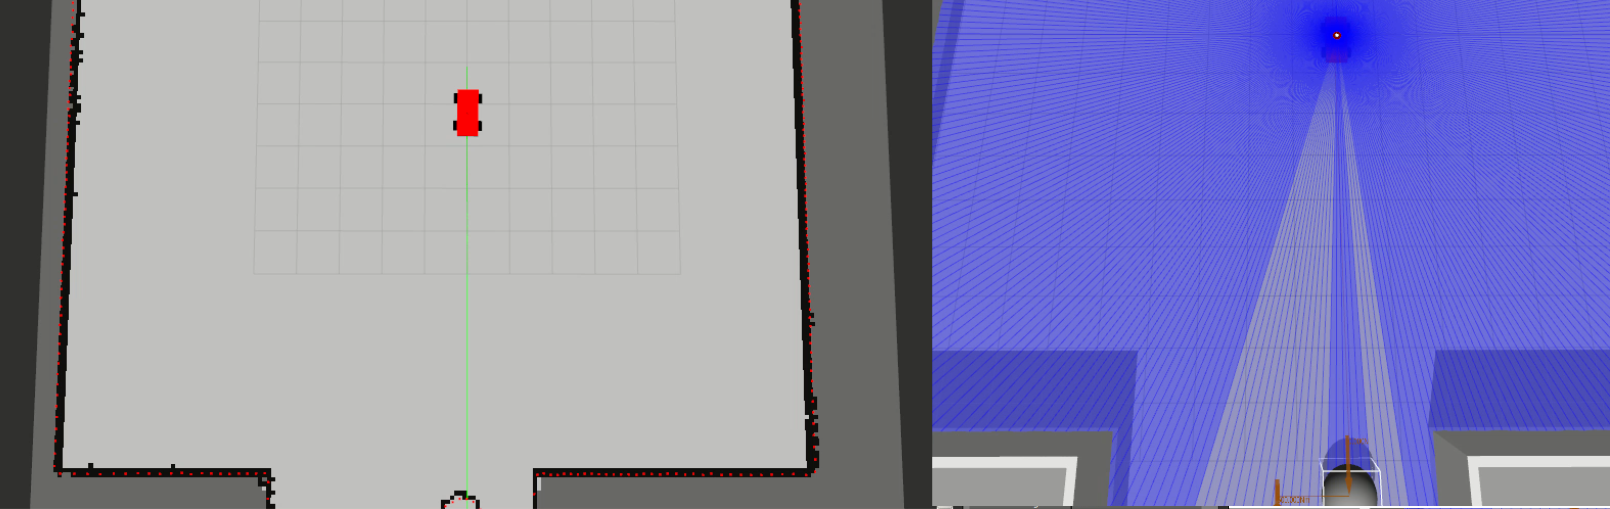
\includegraphics[width=\textwidth]{figures/raw/local_planner_test_straight_traj_dyn_obj_1.png}

	\vspace{0.5cm}
	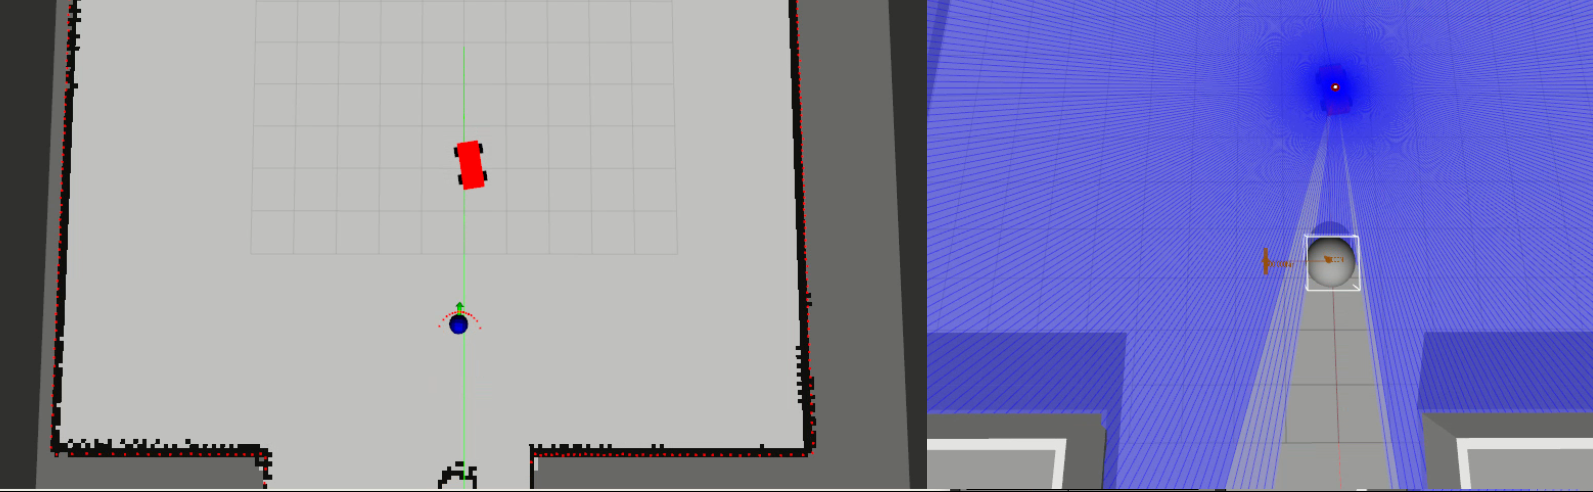
\includegraphics[width=\textwidth]{figures/raw/local_planner_test_straight_traj_dyn_obj_2.png}

	\vspace{0.5cm}
	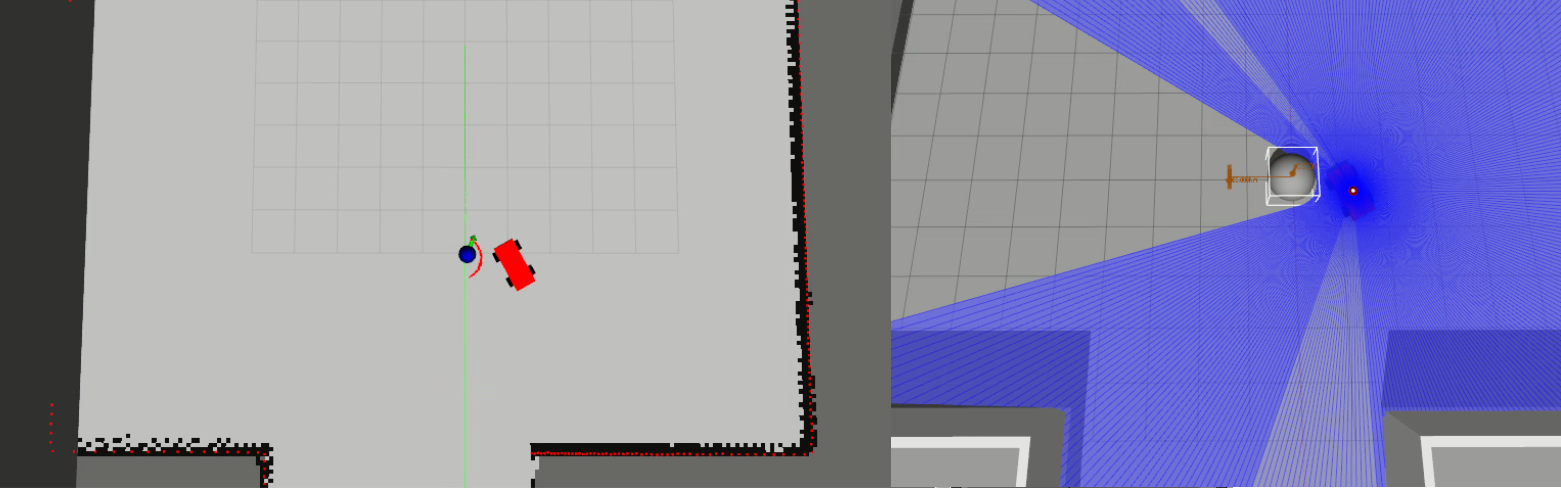
\includegraphics[width=\textwidth]{figures/raw/local_planner_test_straight_traj_dyn_obj_3.png}

	\vspace{0.5cm}
	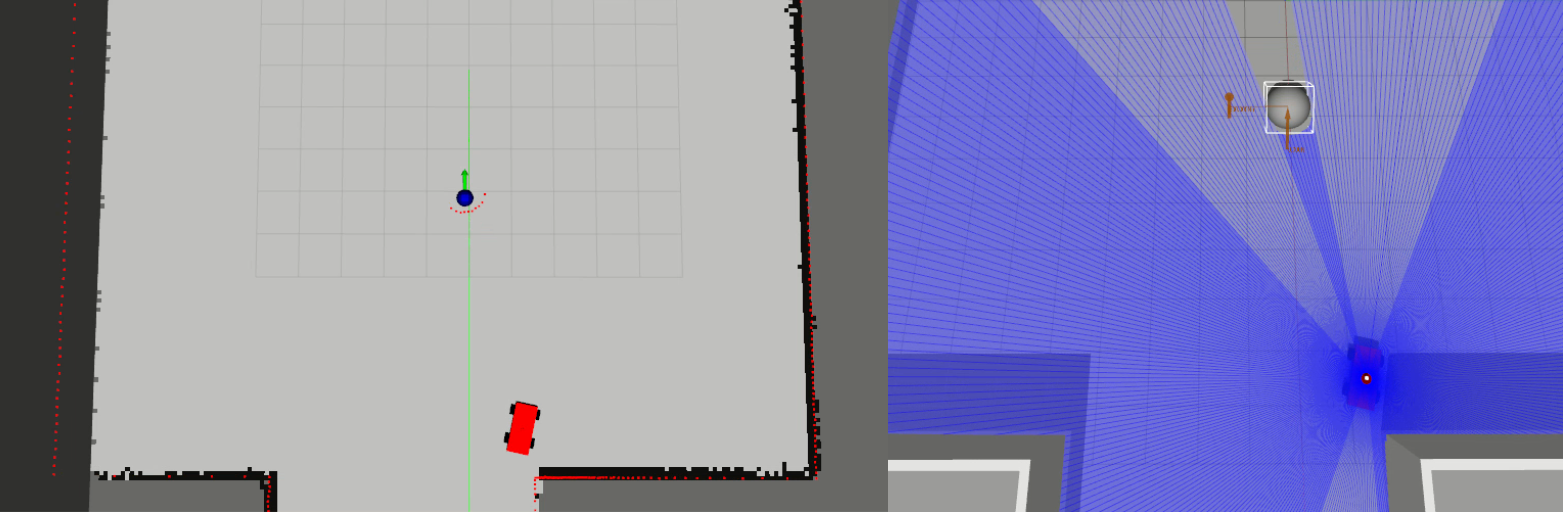
\includegraphics[width=\textwidth]{figures/raw/local_planner_test_straight_traj_dyn_obj_4.png}

	\captionof{figure}{Straight trajectory, dynamic obstacle}
	\label{local_planner_test_straight_traj_dyn_obj}
\end{minipage}

Comparing images \ref{local_planner_test_straight_traj_static_obj}/2 and \ref{local_planner_test_straight_traj_dyn_obj}/2, it clearly shows that in the latter case (when the object is moving opposite the car), the car starts the obstacle avoidance movement a lot earlier. That is because the object is successfully detected as dynamic (marked by a blue circle and a green speed vector in the rviz visualization). A minor deficiency of the algorithm can be seen in figure \ref{local_planner_test_straight_traj_dyn_obj}/3. By the time point represented in the image, the car has successfully avoided the obstacle, but it still keeps to the left. This issue only occurs when the object to pass is moving. The cause of this undesired effect is explained in detail in \ref{chap:closing_ball}. But even with this extra curve, the car successfully keeps to the target path after the collision avoidance.

The scenario represented in figure series \ref{local_planner_test_straight_traj_faster_obj_from_behind} is different from the previous ones in a way. This is the first situation where an actuation that stops the car would cause a collision. That is because in this scenario, a faster object is approaching the vehicle from behind. To prevent a crash, the car must deviate from its original trajectory in order to let the faster obstacle pass by. Then it can continue on its original route again. Personally, this is my favourite scenario of all.

\begin{minipage}{\textwidth}
	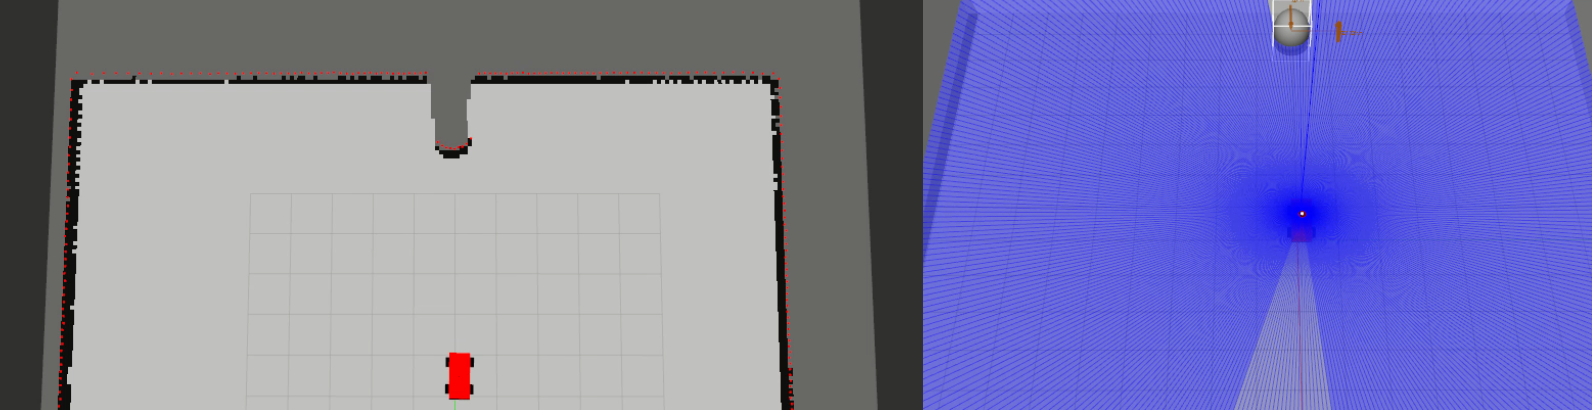
\includegraphics[width=\textwidth]{figures/raw/local_planner_test_straight_traj_faster_obj_from_behind_1.png}

	\vspace{0.5cm}
	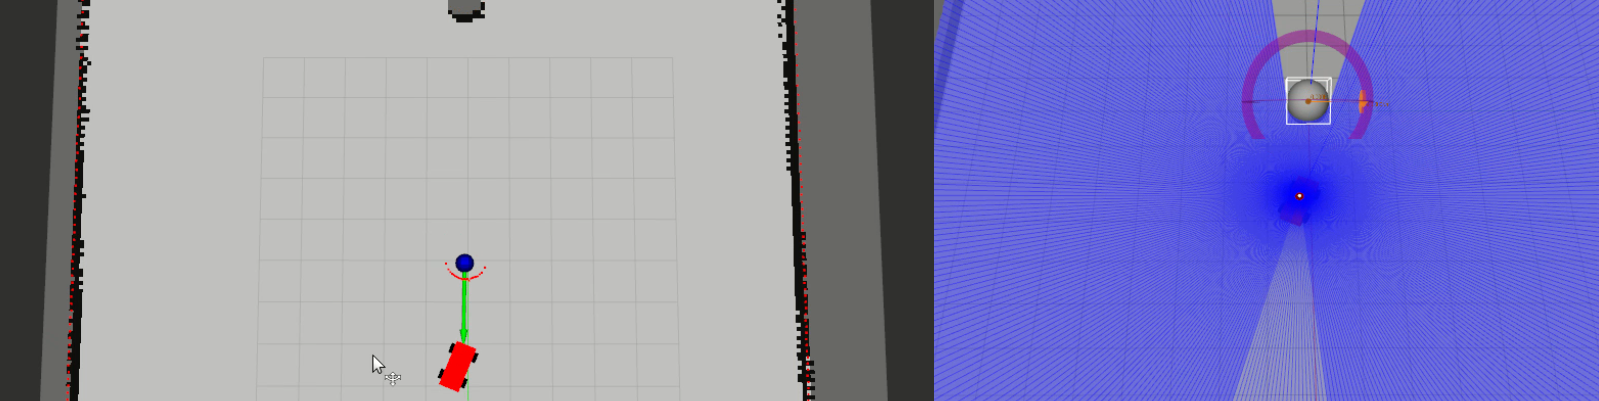
\includegraphics[width=\textwidth]{figures/raw/local_planner_test_straight_traj_faster_obj_from_behind_2.png}

	\vspace{0.5cm}
	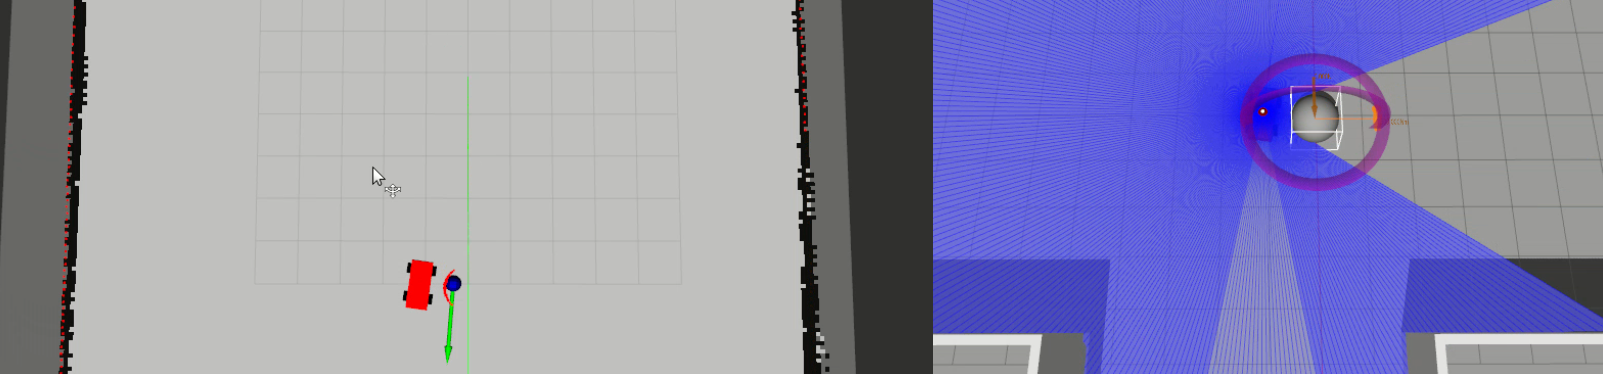
\includegraphics[width=\textwidth]{figures/raw/local_planner_test_straight_traj_faster_obj_from_behind_3.png}

	\vspace{0.5cm}
	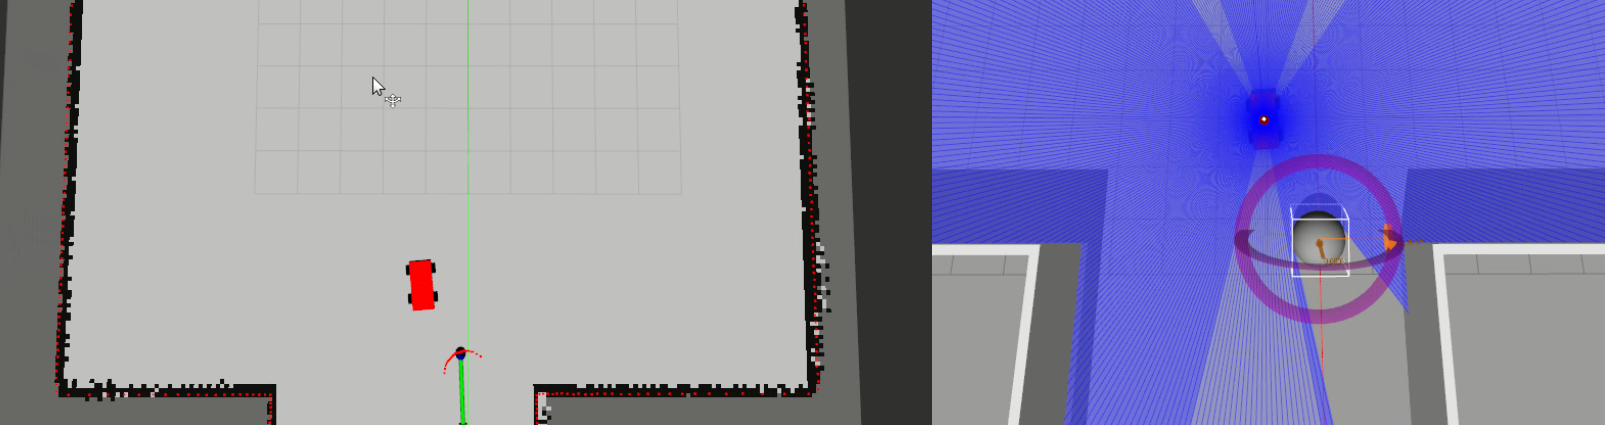
\includegraphics[width=\textwidth]{figures/raw/local_planner_test_straight_traj_faster_obj_from_behind_4.png}

	\captionof{figure}{Straight trajectory, faster obstacle from behind}
	\label{local_planner_test_straight_traj_faster_obj_from_behind}
\end{minipage}

The car detects the possibility of collision in time, and however the offender party would be the other obstacle in case of a crash, the car manages to get out of its way before the collision could happen. After the successful evasion, the car gets back on its original path.

The last example I am going to present points out another deficiency of the algorithm, which is that it does not see the whole path, it only thinks forward for the next couple of meters\footnote{This distance (the length of the virtual string pulling the car towards the destination) is configurable, but optimally is around 4 times the distance between the car's front and rear axles.}. The target trajectory in this example is not a straight line but a series of lines and curves. There are 2 static obstacles in the way (see the right side of the images for the Gazebo simulation).

While the car does manage to avoid both obstacles successfully, it looses the trajectory when circling around the second object. The high-level root of the problem was that the car kept to the right when detecting the obstacle (\ref{local_planner_test_curved_traj_2_static_objects}/4 captures this time snap), instead of turning left, how it would be advised, seeing that the trajectory turns left after the obstacle. Avoiding the object from the right could still be corrected later, if there wasn't a wall behind it that prevented the car from moving forward. This, however, could not have been predicted beforehand, either. The series of these effect caused the car to get in a position where it could not move any further. In these situations, the car stops, a new global trajectory is needed that navigates it out of the trap.

\begin{center}
	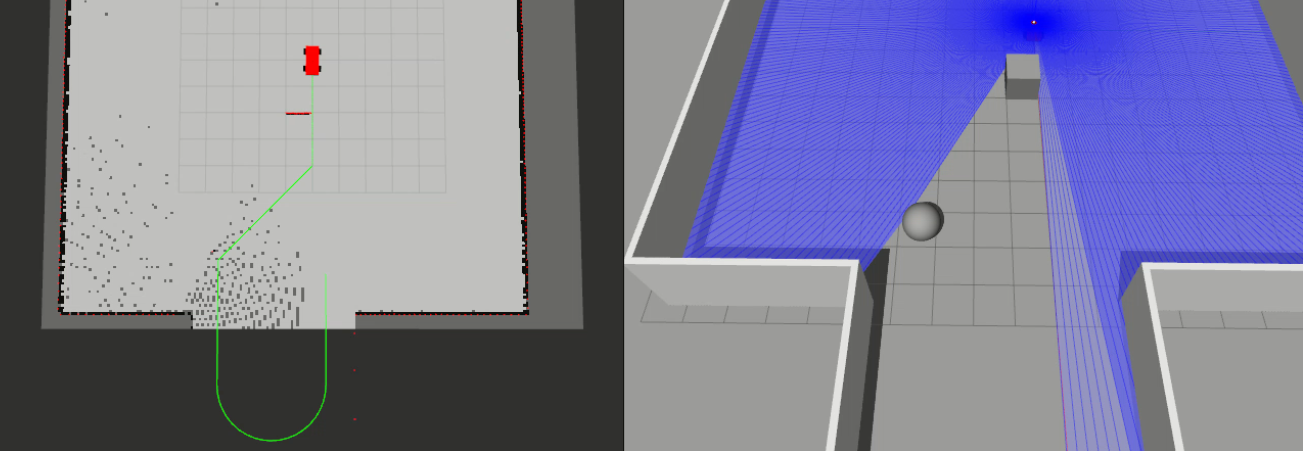
\includegraphics[width=\textwidth]{figures/raw/local_planner_test_curved_traj_2_static_objects_1.png}

	\vspace{0.5cm}
	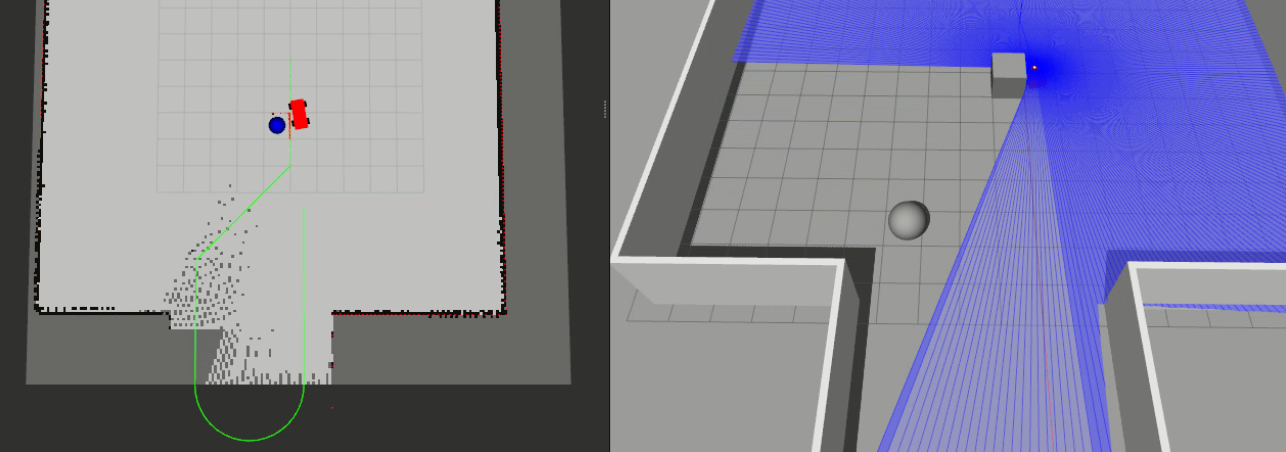
\includegraphics[width=\textwidth]{figures/raw/local_planner_test_curved_traj_2_static_objects_2.png}

	\vspace{0.5cm}
	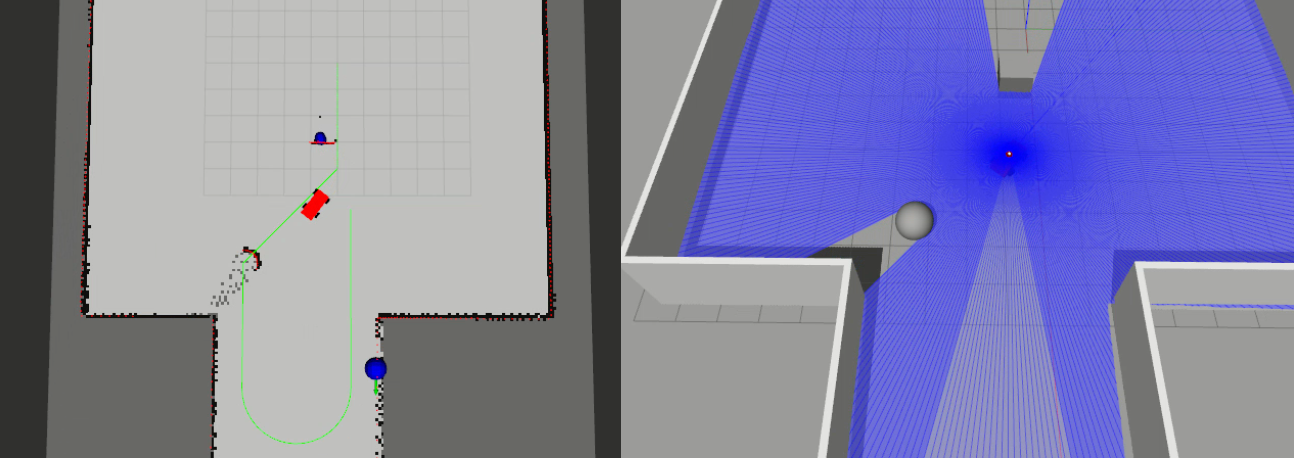
\includegraphics[width=\textwidth]{figures/raw/local_planner_test_curved_traj_2_static_objects_3.png}

	\vspace{0.5cm}
	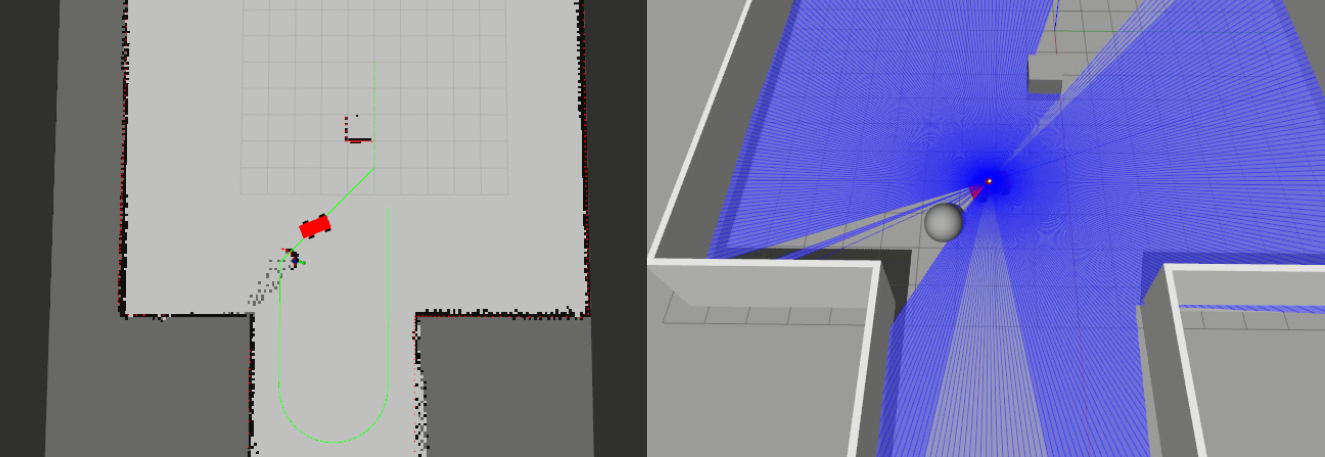
\includegraphics[width=\textwidth]{figures/raw/local_planner_test_curved_traj_2_static_objects_4.png}

	\vspace{0.5cm}
	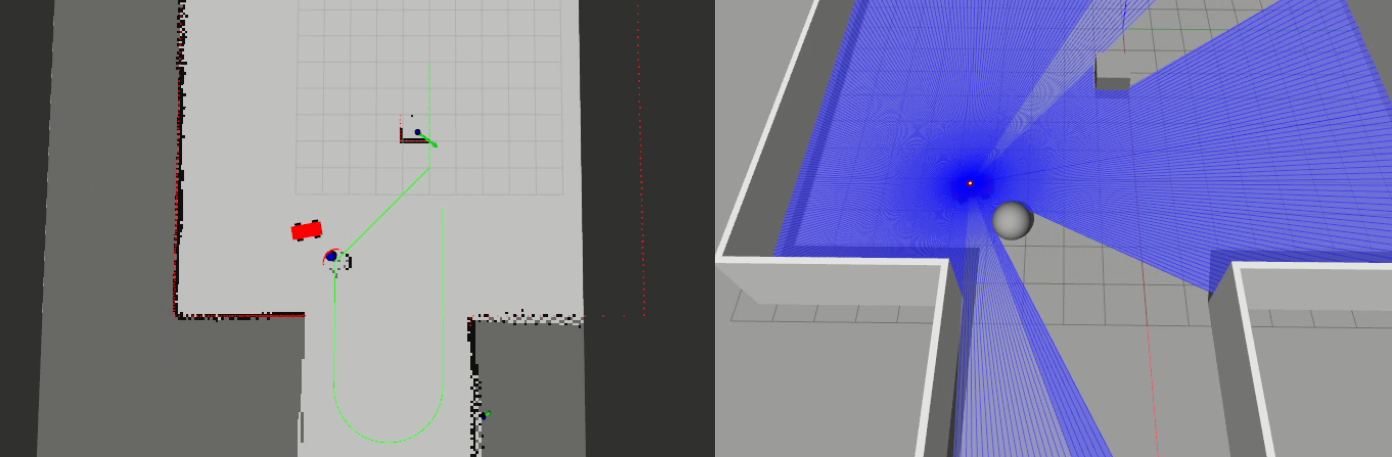
\includegraphics[width=\textwidth]{figures/raw/local_planner_test_curved_traj_2_static_objects_5.png}

	\vspace{0.5cm}
	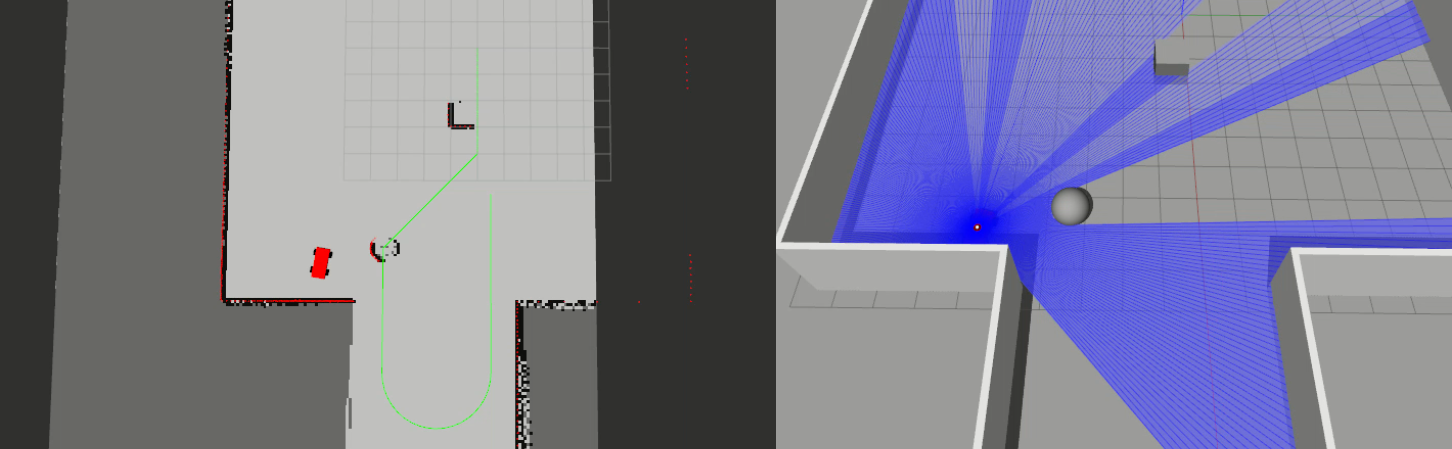
\includegraphics[width=\textwidth]{figures/raw/local_planner_test_curved_traj_2_static_objects_6.png}

	\captionof{figure}{Curved trajectory, 2 static obstacles}
	\label{local_planner_test_curved_traj_2_static_objects}
\end{center}

\subsection{Real-world testing}
\label{chap:real_world_testing}
I tested the above mentioned first two scenarios with the real \textit{vr-car} in a real environment.

In the real world scenarios, the captured video is displayed on the right, while the left side of the image contains the rviz visualization recorded alongside the video footage. The trajectory is always pointing forward, as the videos were captured from behind the car. The rviz visualizations are rotated to match the orientation of the car - so the car is moving upwards in the visualizations.

The first example shows a scenario in which the the car is in a corridor, with a room opening from the it to the right. The target trajectory is straight again (the car needs to navigate through the corridor, keeping to left if possible), but there is a static obstacle in the way. The expected behaviour is to bypass the obstacle from the right, then keep to the left side of the corridor while moving forward.

\begin{minipage}{\textwidth}
	\centering
	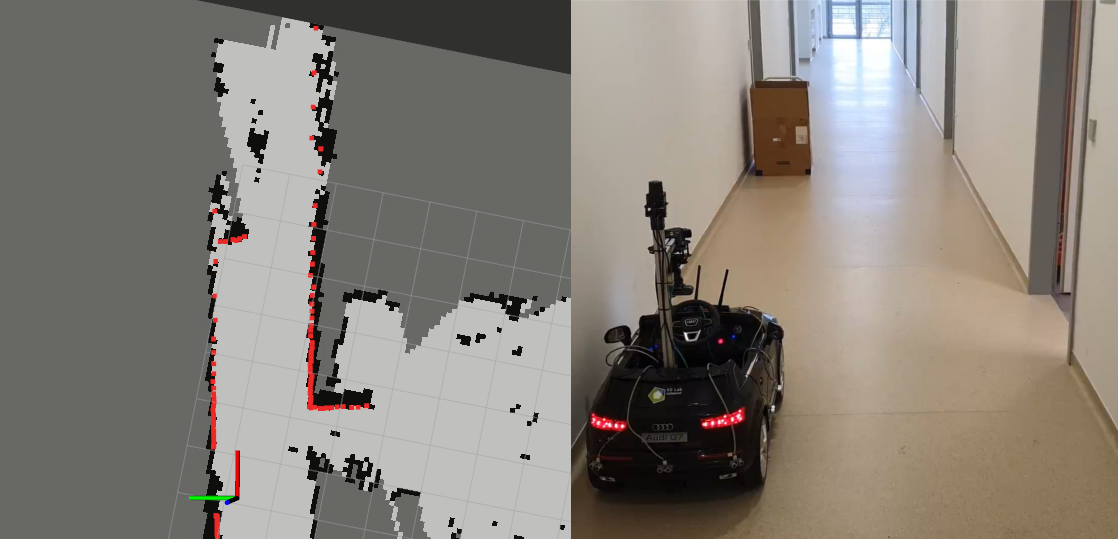
\includegraphics[width=0.65\textwidth]{figures/raw/local_planner_real_test_joined_straight_traj_1_static_obj_1.png}
	
	\vspace{0.5cm}
	\centering
	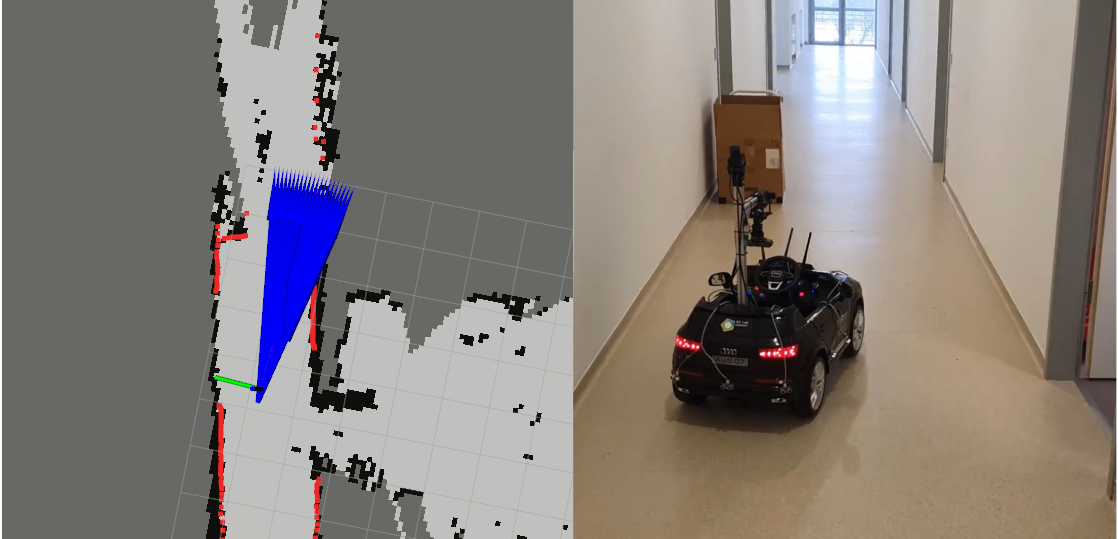
\includegraphics[width=0.65\textwidth]{figures/raw/local_planner_real_test_joined_straight_traj_1_static_obj_2.png}
	
	\vspace{0.5cm}
	\centering
	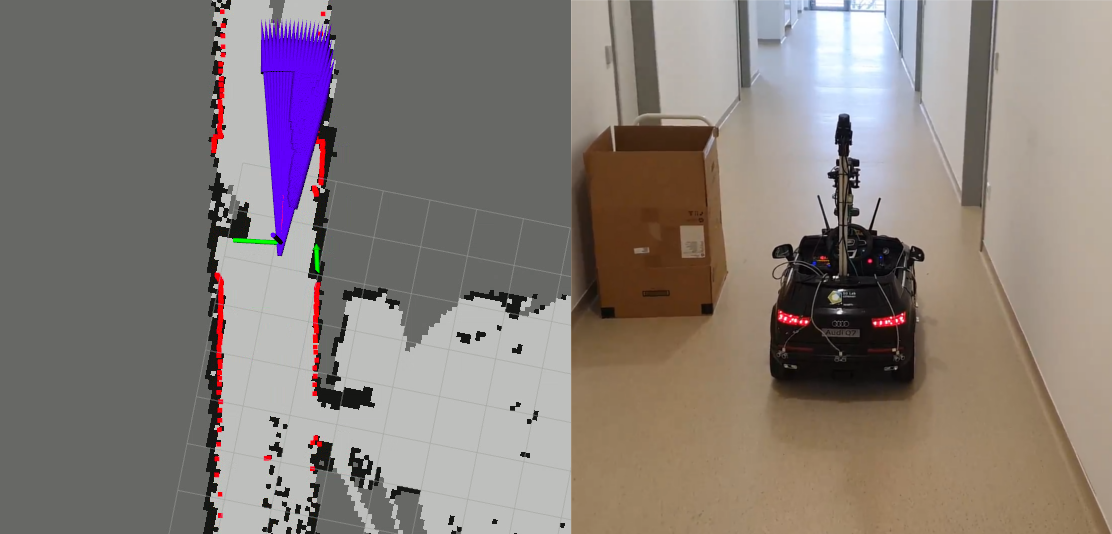
\includegraphics[width=0.65\textwidth]{figures/raw/local_planner_real_test_joined_straight_traj_1_static_obj_3.png}
	
	\vspace{0.5cm}
	\centering
	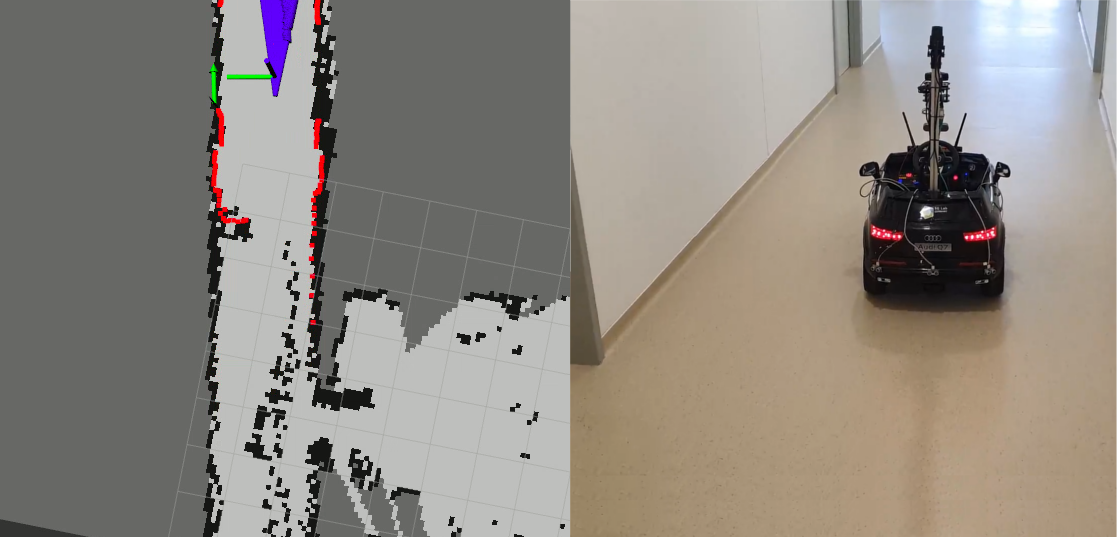
\includegraphics[width=0.65\textwidth]{figures/raw/local_planner_real_test_joined_straight_traj_1_static_obj_4.png}
	
	\captionof{figure}{Straight trajectory, 1 static obstacle}
	\label{local_planner_real_test_joined_straight_traj_1_static_obj}
\end{minipage}

The second example is the same as the previous one but with a dynamic object coming towards the car. For this test, the mapping node had to be started in single LIDAR mode (see SINGLE\_LIDAR in \ref{chap:mapping_input_parameters}) in order to use the scan data provided by the top LIDAR instead of the front and rear ones. This was necessary in order to detect obstacles at a circa 1.2 meter height (above the waist-line). With this modification, the mapping node was able to detect the movement of a human as one solid, linearly moving body, instead of detecting a pair of feet moving non-linearly. 

\begin{center}
	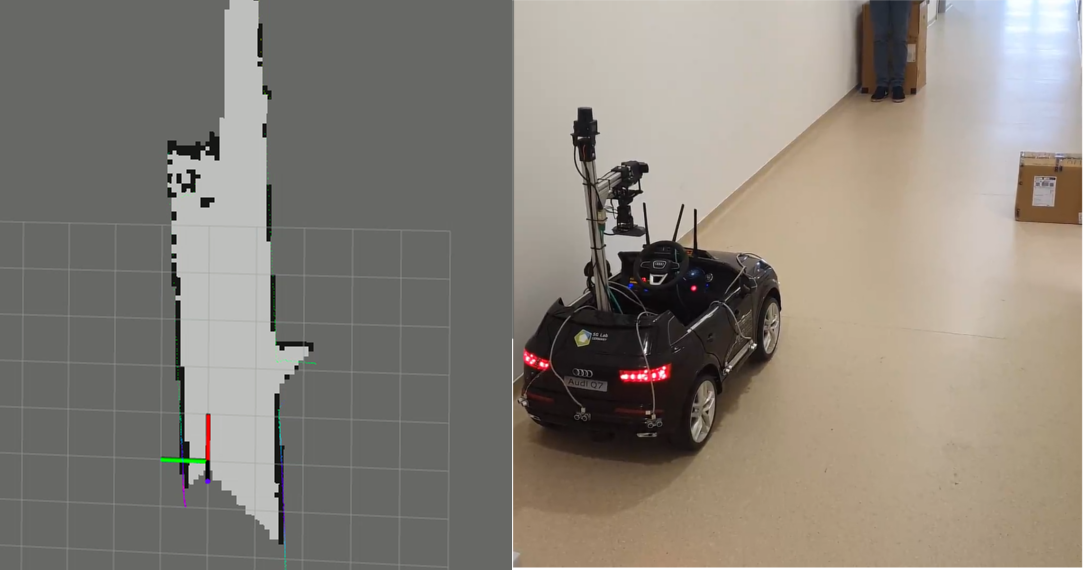
\includegraphics[width=0.65\textwidth]{figures/raw/local_planner_real_test_joined_straight_traj_1_dynamic_obj_1.png}
	
	\vspace{0.5cm}
	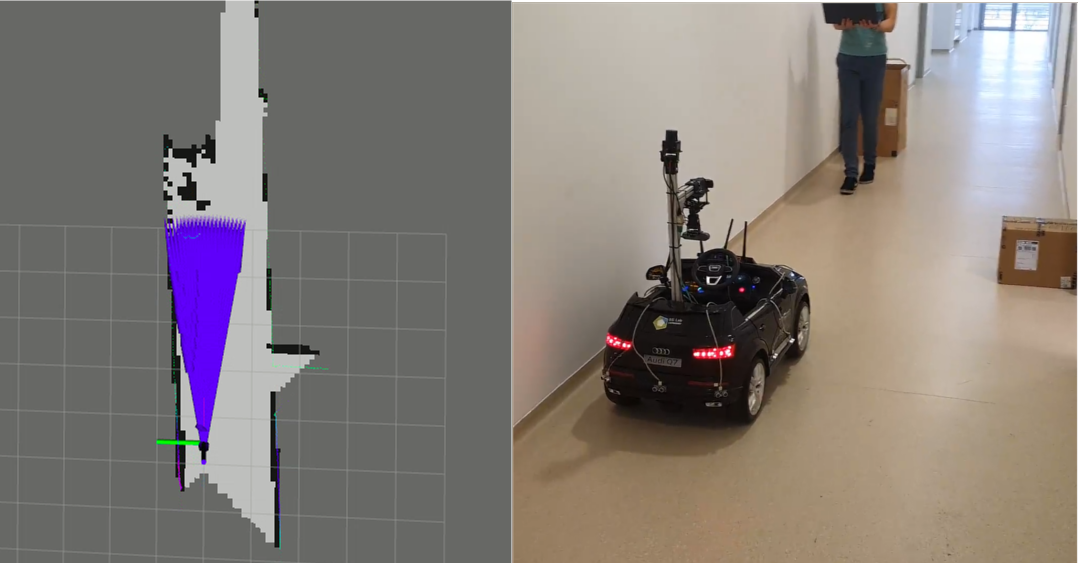
\includegraphics[width=0.65\textwidth]{figures/raw/local_planner_real_test_joined_straight_traj_1_dynamic_obj_2.png}
	
	\vspace{0.5cm}
	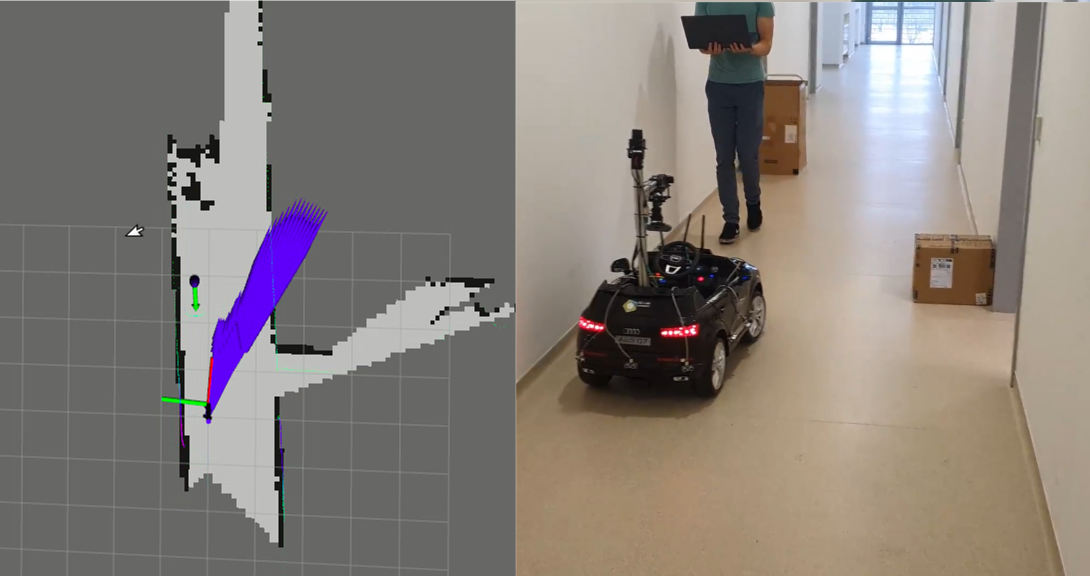
\includegraphics[width=0.65\textwidth]{figures/raw/local_planner_real_test_joined_straight_traj_1_dynamic_obj_3.png}
	
	\vspace{0.5cm}
	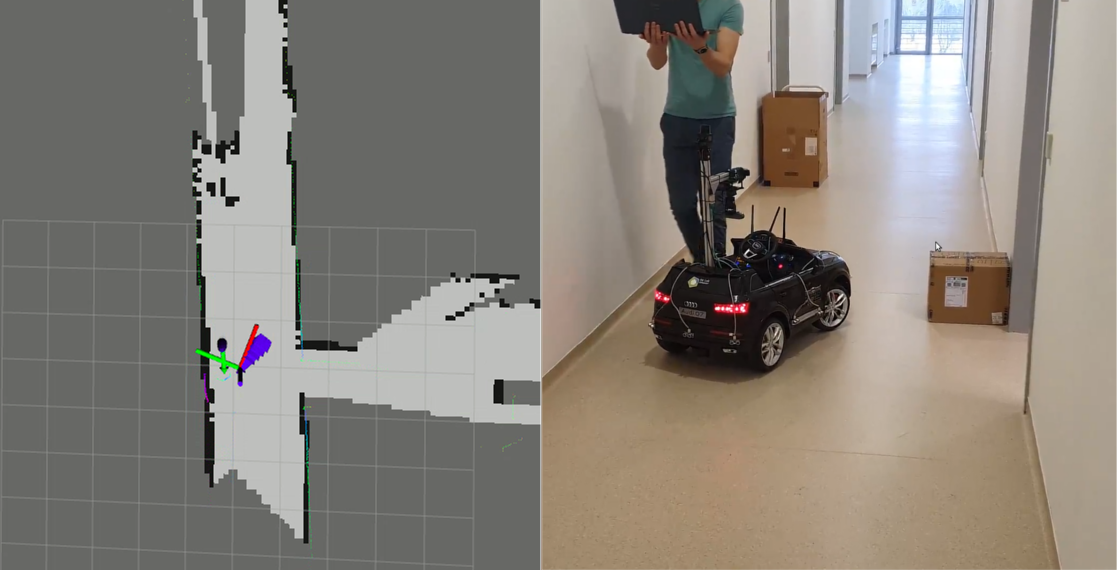
\includegraphics[width=0.65\textwidth]{figures/raw/local_planner_real_test_joined_straight_traj_1_dynamic_obj_4.png}
	
	\vspace{0.5cm}
	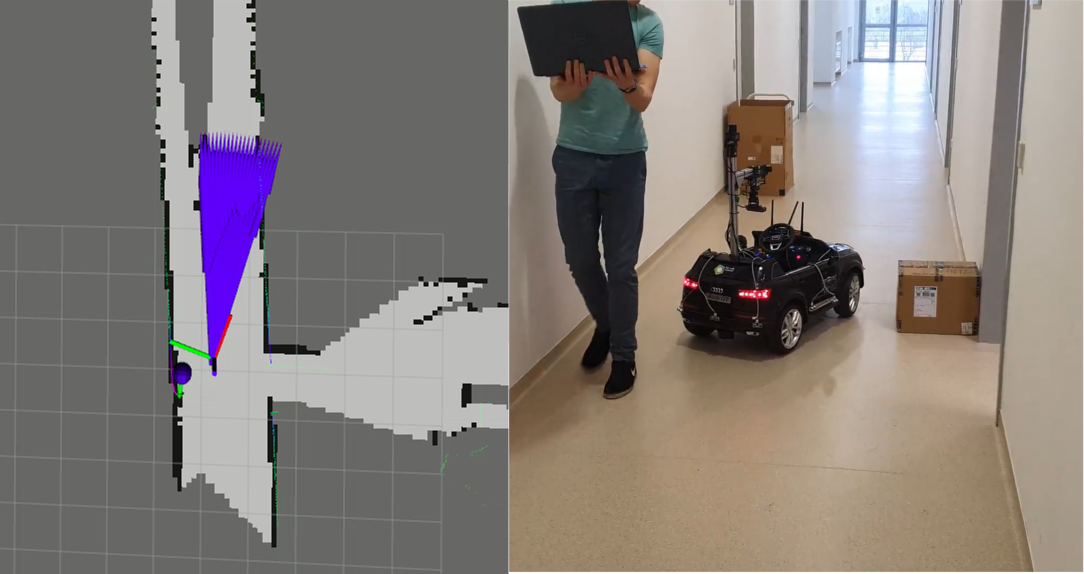
\includegraphics[width=0.65\textwidth]{figures/raw/local_planner_real_test_joined_straight_traj_1_dynamic_obj_5.png}
	
	\vspace{0.5cm}
	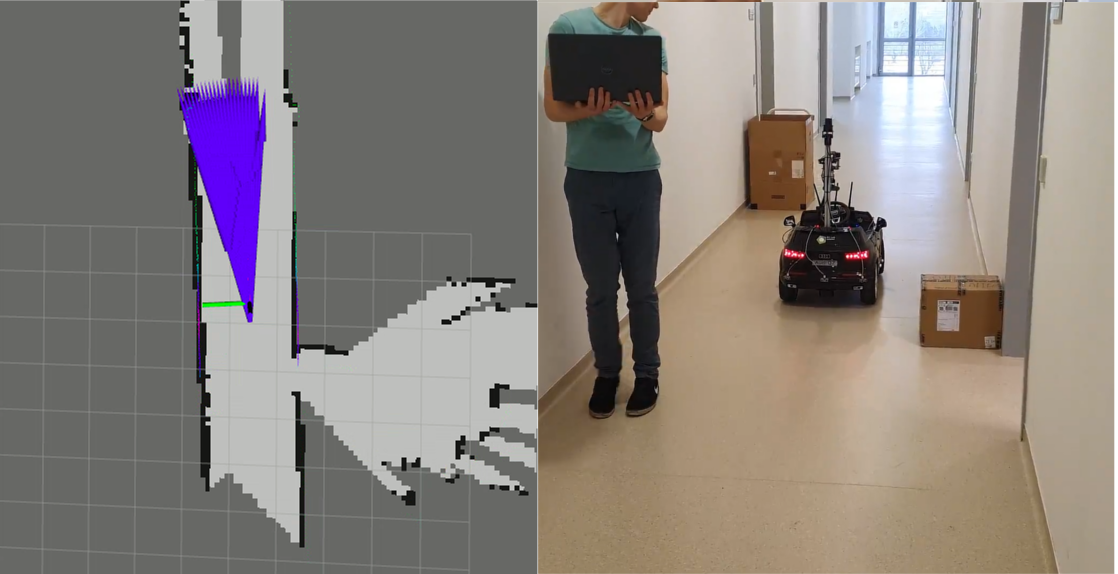
\includegraphics[width=0.65\textwidth]{figures/raw/local_planner_real_test_joined_straight_traj_1_dynamic_obj_6.png}
	
	\captionof{figure}{Straight trajectory, I dynamic obstacle}
	\label{local_planner_real_test_joined_straight_traj_1_dynamic_obj}
\end{center}

The expected behaviour was to bypass the walking obstacle from the right, the same way as in the previous example. The car managed to do that, but it passed so close to the person, that he needed to stop his leg for a moment not to kick the car when being next to it. Note that the minimum kept distance from obstacles is configurable (see MIN\_KEPT\_DISTANCE in \ref{chap:motion_planner_input_parameters}). With the correct tuning of this parameter, these situations can be avoided. Please also note that the above described two real-world tests were the results of several unsuccessful attempts.

An interesting fact for this last scenario is that, due to the top LIDAR being used instead of the ones fixed at ankle-height, short objects (such as the box on the right side of the corridor) are no detected. This is the reason why, by default, the car is using the front and rear LIDARs for obstacle detection and avoidance.